\documentclass[12pt]{article}
\usepackage{epsfig,wrapfig,url,palatino,color,graphicx}
\usepackage{caption}
\usepackage{subcaption}
\graphicspath{{images/}}
 

\pagestyle{plain}
\renewcommand{\baselinestretch}{1.}

\setlength{\topmargin}{0in}
\setlength{\evensidemargin}{0in}
\setlength{\oddsidemargin}{0in}
\setlength{\headheight}{0in}
\setlength{\headsep}{0in}
\setlength{\footskip}{0.2in}
\setlength{\textheight}{9in}
\setlength{\textwidth}{6.5in}

\renewcommand{\topfraction}{0.99}
\renewcommand{\bottomfraction}{0.99}
\renewcommand{\textfraction}{0.01}
\renewcommand{\floatpagefraction}{0.01}
\renewcommand{\dbltopfraction}{0.99}
\renewcommand{\dblfloatpagefraction}{0.01}

\begin{document}

\noindent
{\bf Title of Proposal:} Evaluation of the usability of a web based 
sketching interface for the iterative design of architectural daylighting \\
{\bf Researcher:}   Max Espinoza\\
{\bf Address:}  MRC 311\\
{\bf Phone:} 518 276 3274\\ 
{\bf Research Advisor (for students):}  Barbara Cutler \\
{\bf Department:}  Computer Science \\
{\bf Is this proposal related to a sponsored project?}  Yes \\
{\bf If yes,  please indicate:}  \\
Existing Award: (Fund \# A12016), NSF, \\
Immersive Architectural Daylighting Design Experience \\

\noindent
All investigators, including faculty supervisors, on this project must
complete the self-study course on protection of human research
subjects. \\
{\bf Certification:  I/We have completed the course:} \\
Max Espinoza (CS PhD Student) 10/05/15 \\ 
Barbara M Cutler 7/2/08, refresher 11/2/11 % Might get complaints about not up to date refresher

\paragraph{Objective:}
%
Our goal in this study is to evaluate the effectiveness and usability of 
our web based sketching interface for the creation of closed architectural 
geometries and daylighting analysis.

\paragraph{Methods:}
%
Users in our study will begin by visiting a provided URL serviced by a password protected lab machine.
Users will be required to register by providing a username of their choice and a password.
During registration users will be given a brief explanation of their participation in our
user study. There will also be an option to opt out of the user study, but still use our web interface. 
This opt out option will be clearly displayed when registering for our web application.
We will not use designs or feedback of users who have opted out of the study.
A sample screenshot of the registration process is shown below.
After a successful login users will then be taken the main page of our application.
The application is split into two parts. On the left hand side are the tools required to
make sketches and generate 3D models. On the right hand side is a feedback panel with question 
that can be answered at any point of the study. These questions are not required to be answered in order
to use the web interface. Users can choose to answer some questions, but leave others blank.
Participants can stop at any point in time and continue by logging into the web interface
with their username and password.\\

\noindent
The questions asked are attached at the end of this document. (Along with sample screenshots)

\paragraph{Effects on Subjects:} See benefits and risks.

\paragraph{Benefits to Participants:}
%
The participants will gain first-hand experience with a new online sketching
environment for the generation of 3D models, and an understanding of the 
iterative design process of creating architectural spaces. The results 
of the study will lead to the use, development, and improvement of algorithms that
interpret architectural sketches. In addition user's feedback will lead to 
improvements in our daylighting visualizations.


\paragraph{Minimization of Possible Risks:}   
% 
There is no rick of physical harm in our web interface study. 
The only tool required to participate in this study is a computer and webbrowser.
We have considered the issue of computer security. Users will provided two kinds 
of digital information: design files and feedback. 
Design files are created automatically as the participants uses our interface. 
These files save user's sketches in a format that is unique to our interface.
To protect users we have a login system that requires a unique username and password pair. Users will be able to
revisit the website to review/edit design files and feedback.
The application is designed to store information created by users on a PostgreSQL 
database serviced by the Computer Science Department, of which only investigators have direct access to.
The machine hosting this webpage will be using an up to date Apache server and hypertext transfer protocol secure (HTTPS)
for maximal security. We will also hash user's password, such that no where on the system will
user's passwords be stored in plain text.
Users are not required to download anything on their computers to participate in this study, nor will
they be required to make security exceptions on firewalls or anti-virus protection software.
Our webpage is only dependent on users having a webbrowser (Firefox or Chrome) to participate.

\noindent
The answers to some questions may contain personally identifiable information.
For example participant are asked to identify what room they are creating a sketch of, more over users are asked how often they visit this room.
All the questions in our survey are optional, including those questions which may contain personally identifiable information.

\paragraph{Likelihood of  Harm:}   None
\paragraph{Alternate Method Not Using Human Subjects:} None

\paragraph{Qualifications of Researcher:}
Barbara Cutler has a PhD in Computer Science from Massachusetts
Institute of Technology.  Max Espinoza is a 3th year PhD student in
Computer Science at Rensselaer Polytechnic Institute studying computer
graphics.

\paragraph{Recruiting of Subjects:}
We will ask for online volunteers to use our webpage and participate in this
user study. We will advertise our web page to student volunteers (18 years or older) 
via posters, campus related social media, and direct contact with students attending 
related courses. We will obtain permission of the course instructors to advertise 
for the participation of their students, but participation in the study will be 
voluntary and will not impact their course grade. The faculty advisor for the 
study (Barbara Cutler) will not recruit students in her courses to participate.  
The names of the students who did or did not participate in the study will be 
confidential and will not be released to their instructors.

We are particularly interested in participants with experience in 3D modeling, 
architectural daylighting, general architecture, and visual arts. We are looking 
for users with formal education and experience in the above fields to provide 
us valuable feedback to improve our web interface's usability and functionality. 
This experience is not required for participation in the user study, but the 
subject's will have an opportunity to note prior experience in these related fields.

\paragraph{Confidentiality:} 
Participants will register themselves with a username of their choice,
when logging into the web interface for the first time. 
We do not require users to use any personally identified usernames and password pairs such as those provided by
the RPI (RSC IDs). We work under the assumption that users follow standard practices for the creation 
and management of their login credential's.
The participates can stop and continue where they left off at any point during this study using their
unique usernames. Users will also provide a password, which we will hash using SHA-1 method. 
This hashed password is used to protect user's design file and
feedback information. No where in our application will the user be asked for their real 
name. Participants will be identified by a randomly assigned ID number that is used only for 
this study. All recorded user information and design files will be labeled with this ID 
(and not the participant's username). All information and data relating to the user study 
will be protected to secure confidentiality. All electronic files will be stored on password 
protected computers in locked offices, which can be accessed only by the investigators of 
the user study. The correspondence between ID number and participant username will be recorded 
by Barbara Cutler and stored on a password protected computer, accessible only by her. 
This correspondence will be destroyed once analysis of the data is complete, within 1 year 
after participation in the study.

\newpage
\paragraph{Registration and Login Sample:}
When users visit our URL they will be directed to a registration page. Users who have already previously registered can navigate another page to sign in. Screenshots of the registration page are provided below. On this page users are only required to provide a username and password. In addition there is a brief prompt explaining what information is being recorded and an option to opt out of this study. All other kinds of user input beyond this point are optional.

\begin{figure}[h]

  \begin{subfigure}{.5\textwidth}
    \centering
    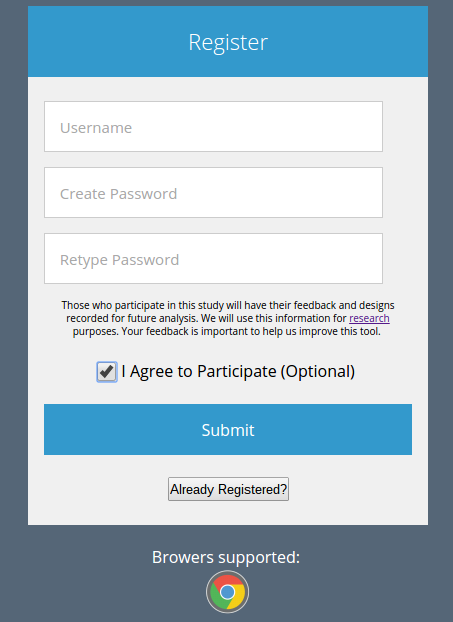
\includegraphics[scale=0.5]{ss_reg}
    \caption{This is the registration page for new user. Note the brief statement regarding participation in our user study.}
  \end{subfigure}%
  \begin{subfigure}{.5\textwidth}
    \centering
    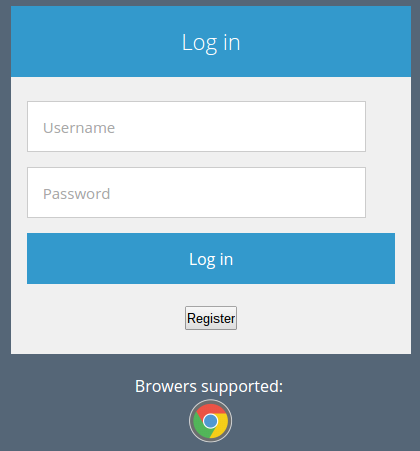
\includegraphics[scale=0.5]{ss_sign}
    \caption{Sign in prompt}
  \end{subfigure}

\caption{Registration and Sign in pages}
\end{figure}

\newpage
\paragraph{Sample User Specific Questions:}
These are sample questions we will ask on a per user basis. All of these
questions are optional. Screenshots of where these questions are presented in our website are provided below.

\begin{figure}[h]
\centering
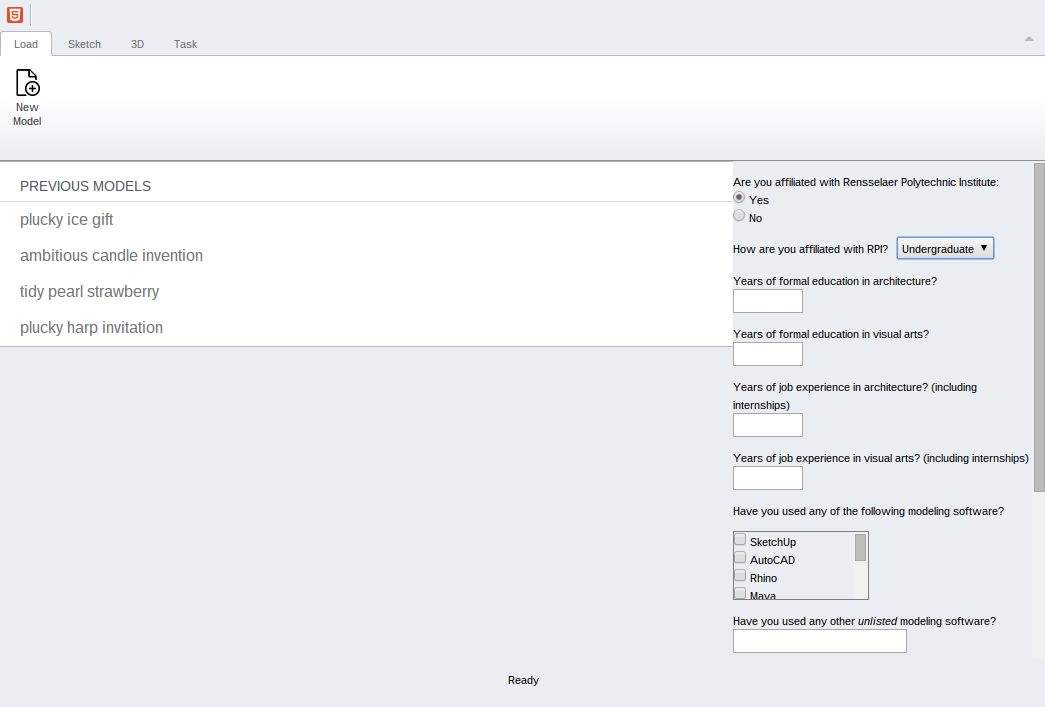
\includegraphics[scale=0.4]{ss_load}
\caption{This is the main page of our interface. Notice the questions users are encouraged to answer are located only the right hand side of the webpage.}
\label{fig:sfig1}
\end{figure}

\begin{enumerate}  
        \item Are you affiliated with Rensselaer Polytechnic Institute? 
        \item How are you affiliated with Rensselaer Polytechnic Institute?
        \item Years of formal education in Architecture?
        \item Years of formal education in Visual Arts?
        \item Years of job experience in architecture? (including internships) 
        \item Years of job experience in Visual Arts? (including internships)
        \item Have you used any of the following modeling software?
        \begin{enumerate}  
          \item SketchUp
          \item AutoCAD
          \item Rhino
          \item Maya
          \item 3DS Max
          \item Cinema 4D
          \item Blender
          \item Revit
          \item Other
        \end{enumerate}
        \item Years of experience with modeling software?
        \item Other relevant education / experience?
        \item Are you colorblind?
        \item Is it okay if we follow up with additional questions about specific models you created in our system?
          \begin{enumerate}
            \item If so, please enter your email address
          \end{enumerate}

    \item What did you find fun or interesting in this sketching environment?
    \item What additional features should be added to system to allow greater flexibility in design?
    \item Describe some designs that you were not able to create due  to system limitations?
    \item Was there anything you did not like about working in this sketching environment?
    \item Where there any UI elements that were hard to use or confusing at first?

    \item Describe your overall impression of the software for determining the interior vs exterior space in your designs?
    \item For the cases when the system’s interpretation of the interior/exterior of your design was incorrect where was the system wrong? 
    \item Did you understand the results of the simulation, was there anything confusing or unclear?
    \item Did the system allow you to create and test daylighting performance with respect to over or under illumination?

      \end{enumerate}

\newpage

\paragraph{Design Specific Sample Questions:}
These are sample questions we will ask on a per design basis.
Upon the creation of a design these questions will be available for users to answer.
Again all of these questions are optional.
Some of these questions ask users for possibly personally identifiable information, however participants are not required to answer these questions. We remind users that these questions are optional by labeling them as optional.
Screenshots of where these questions are presented in our website are provided below.

\begin{figure}[h]
  \begin{subfigure}{.5\textwidth}
    \centering
    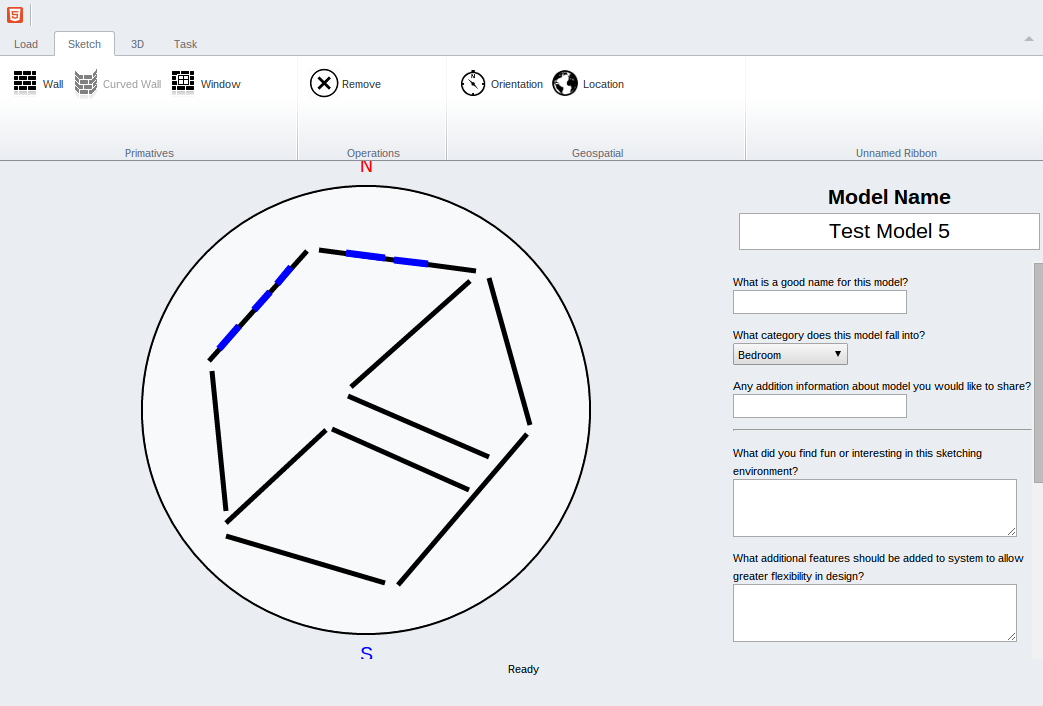
\includegraphics[scale=0.2]{ss_sketch}
    %\caption{Users will create simple designs here by dragging lines across the screen. These designs in addition to feed back are saved for future analysis.}
    %\label{fig:sfig1}
  \end{subfigure}%
  \begin{subfigure}{.5\textwidth}
    \centering
    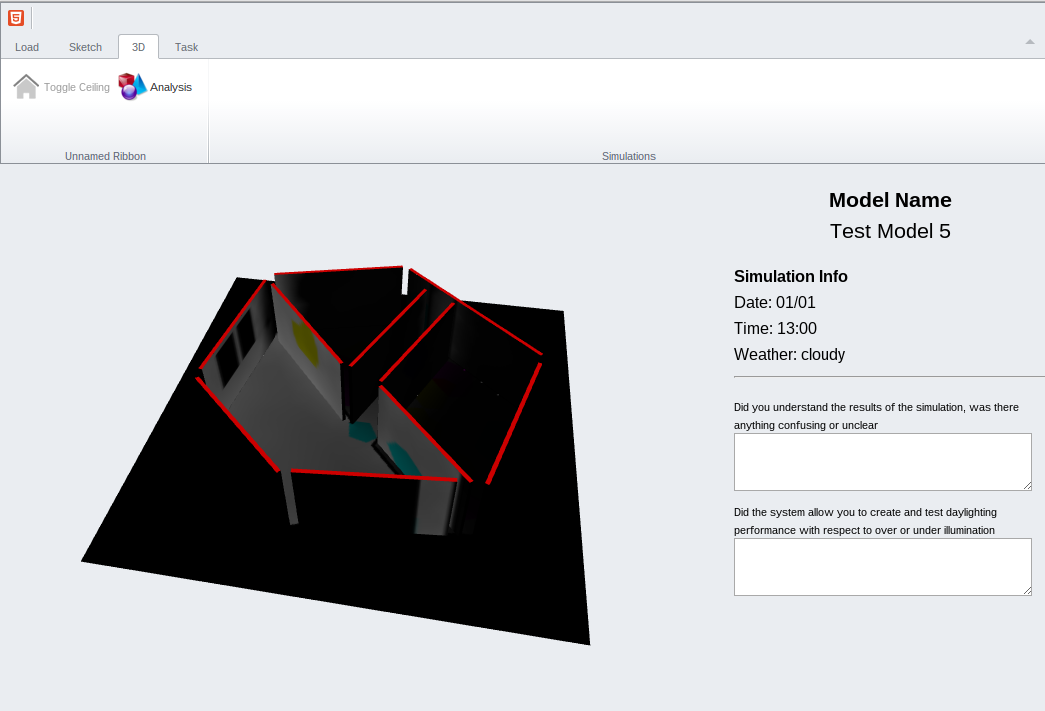
\includegraphics[scale=0.2]{ss_render}
    %\caption{Users visualize the 3D rendering of their designs here. }
    %\label{fig:sfig2}
  \end{subfigure}
\caption{Left) This is sketching interface where users create designs. These designs are recorded for future analysis. Right) Users can view the daylighting of their 3D generated designs. Notice how throughout the application the feedback we are collecting is non-intrusive and located on the right hand side. }
%\label{fig:fig}
\end{figure}

      \begin{enumerate}
        \item What category does this model fall into?
        \begin{enumerate}
          \item Dorm
          \item Bedroom
          \item Living room 
          \item Apartment / House
          \item Classroom
          \item Office
          \item Lobby
          \item Other
        \end{enumerate}
        % If it is an rpi dorm 
      \item What dorm is this a model of? (Optional)
      \begin{enumerate}
        \item BARH (Burdett Avenue Residence Hall)
        \item Barton Hall
        \item Beman Lane Undergraduate RAHP Apartments
        \item Blitman Residence Commons
        \item Bray Hall
        \item Bryckwyck Floor Plans
        \item Cary Hall
        \item Colonie Apartments
        \item Commons
        \item Crockett Hall
        \item Davison Hall
        \item E-Complex
        \item Hall Hall
        \item Nason Hall
        \item North Hall
        \item Nugent Hall
        \item Quadrangle (The Quad)
        \item Sharp Hall
        \item Single RAHP
        \item Stacwyck Apartments
        \item Warren Hall
        \item Other
      \end{enumerate}
    \item What floor number? (Optional)
    \item What room number? (Optional)
    \item When was the last time you visited this space? (Optional)
      \begin{enumerate}
        \item Less than a week ago
        \item Less than a month ago
        \item Less then a year ago
        \item Less than 4 years ago
        \item More than 4 years ago
      \end{enumerate}
    \item How often did you visit this space?
      \begin{enumerate}
        \item Once
        \item Occasionally
        \item Multiple times a week
      \end{enumerate}
    \item How confident are you in modeling this space? (scale of 1 to 5)
    \item Does the 3D generated model match your intentions?
      \begin{enumerate}
        \item Matched my intentions exactly ( no revision required )
        \item Did not match my intentions initially ( revisions were required )
        \item Failed to match my intentions ( even after revision )
      \end{enumerate}
  \end{enumerate}

\newpage 

\end{document}
